\chapter{System Design}

\section{Introduction}

This chapter presents the comprehensive system design for JKart, translating requirements into architectural decisions, component designs, data models, and API specifications. The design follows microservices patterns with Spring Cloud infrastructure and MongoDB data persistence.

\section{Architectural Design}

\subsection{High-Level Architecture}

JKart implements a three-tier architecture:

\begin{enumerate}
    \item \textbf{Presentation Layer:} React.js single-page application providing user interface for customers and administrators
    \item \textbf{Application Layer:} Nine Spring Boot microservices implementing business logic
    \item \textbf{Infrastructure Layer:} MongoDB databases, AWS EKS, service discovery, API gateway
\end{enumerate}

The React frontend communicates exclusively with the API Gateway (port 8080), which routes requests to backend services based on URL patterns:
\begin{itemize}
    \item \texttt{/api/auth/**} $\rightarrow$ Auth Service (9030)
    \item \texttt{/api/user/**} $\rightarrow$ User Service (9050)
    \item \texttt{/api/category/**} $\rightarrow$ Category Service (9000)
    \item \texttt{/api/product/**} $\rightarrow$ Product Service (9010)
    \item \texttt{/api/cart/**} $\rightarrow$ Cart Service (9060)
    \item \texttt{/api/order/**} $\rightarrow$ Order Service (9070)
    \item \texttt{/api/notification/**} $\rightarrow$ Notification Service (9020)
\end{itemize}

\begin{figure}[h!]
\centering
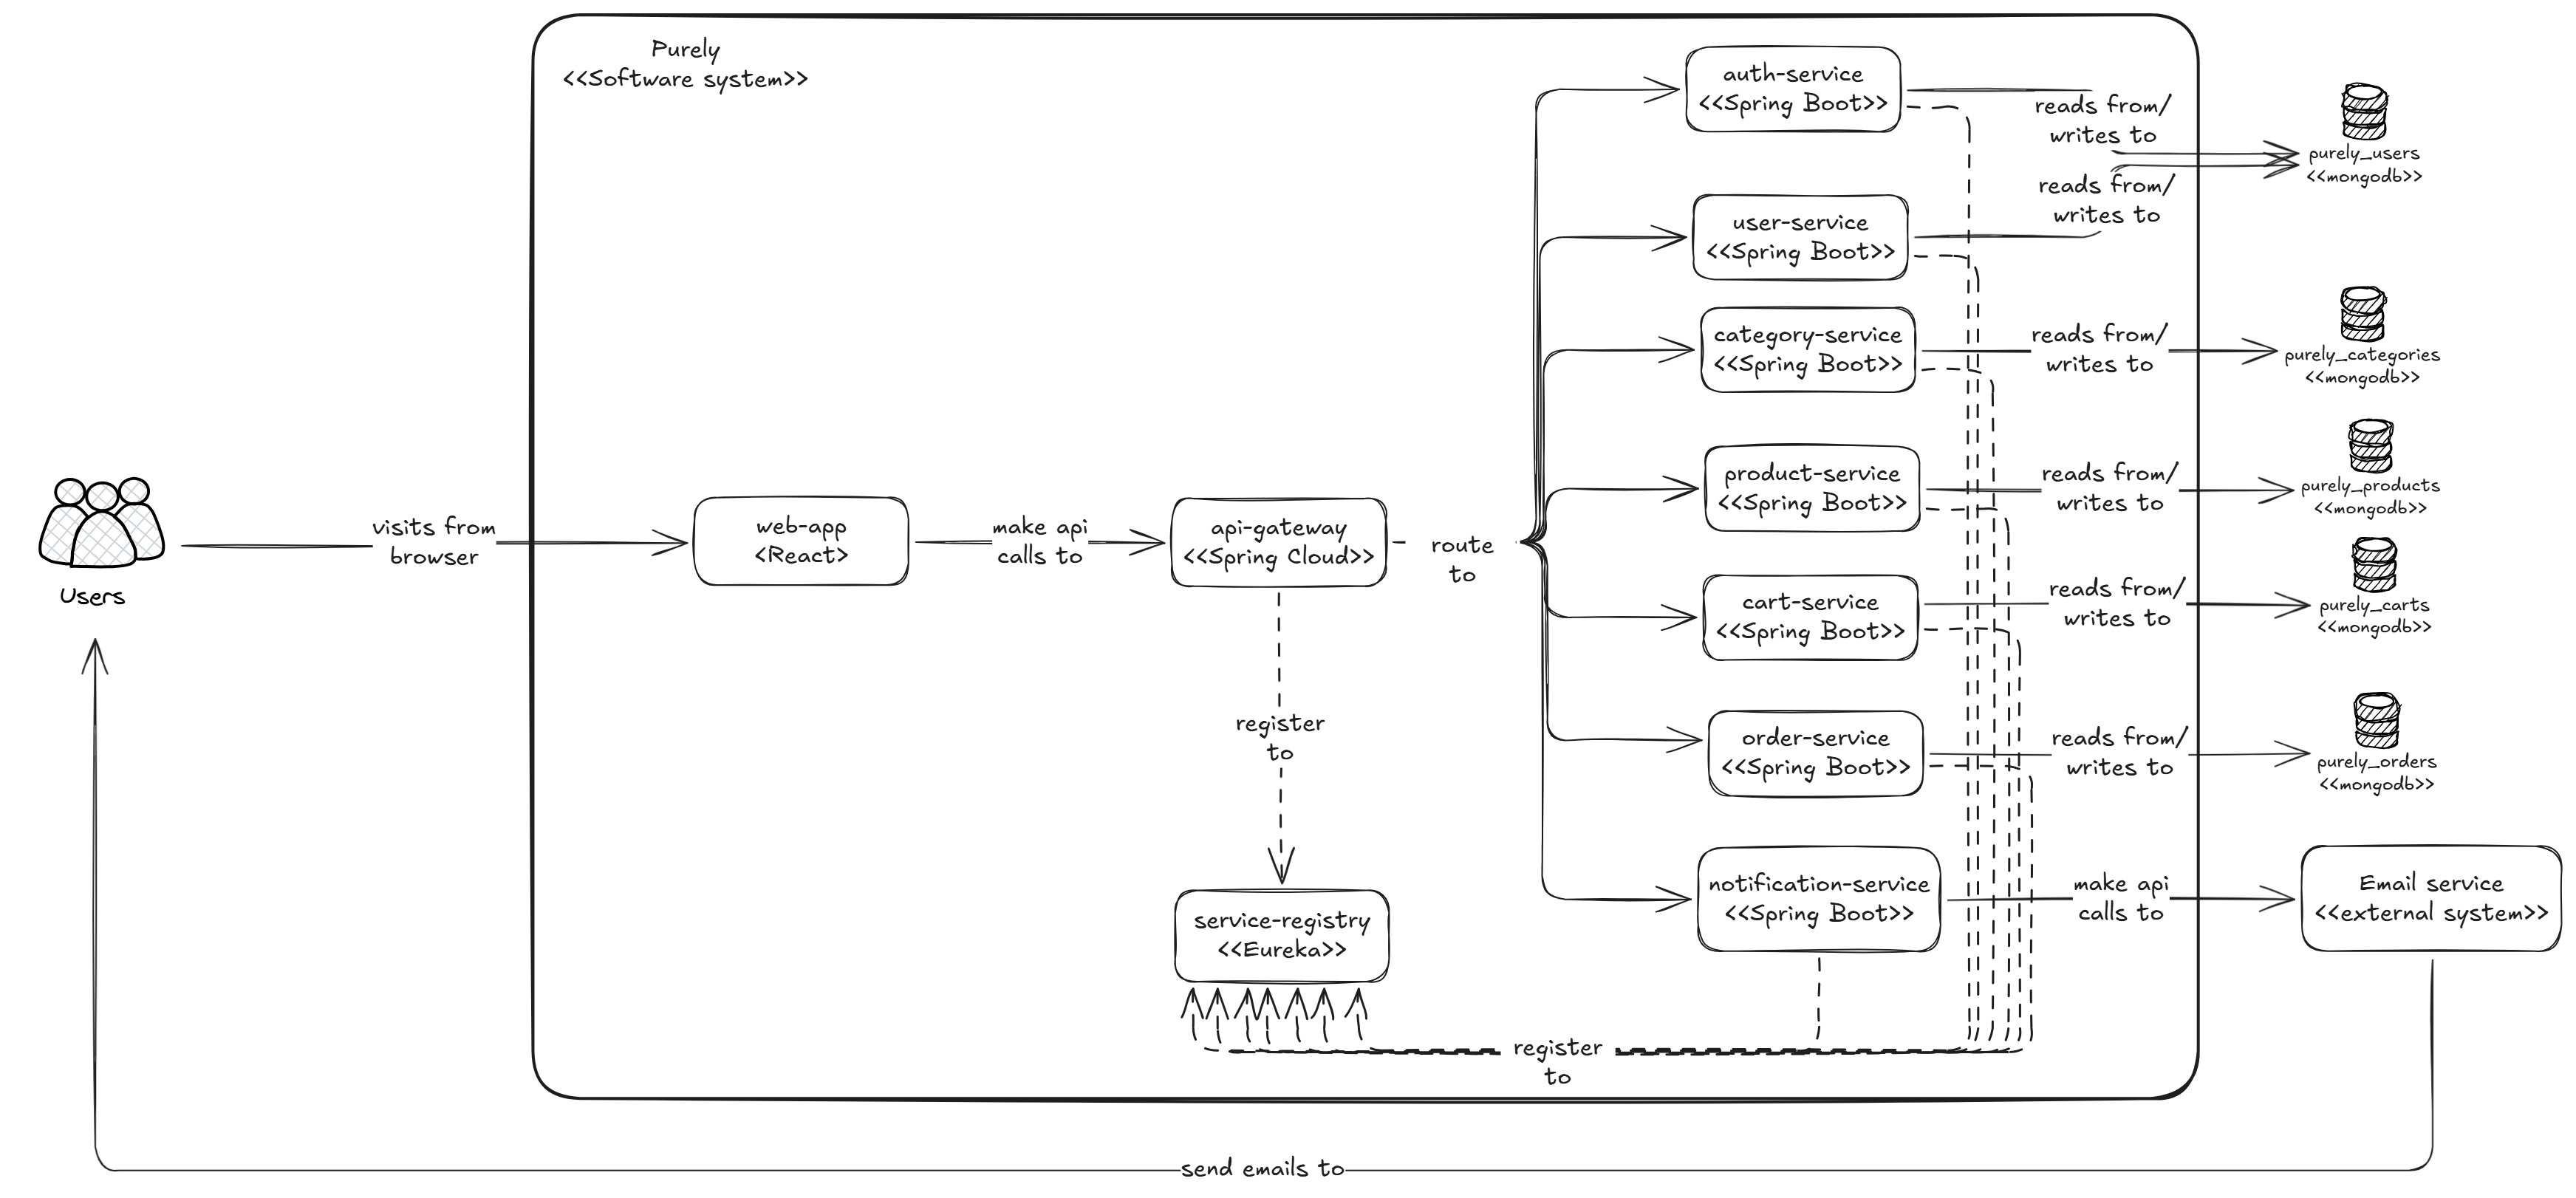
\includegraphics[width=0.85\textwidth]{component_diagram.png}
\caption{JKart Microservices Architecture Component Diagram}
\label{fig:component}
\end{figure}

\subsection{Service Decomposition}

Services are decomposed by business domain following Domain-Driven Design:

\textbf{Service Registry (Eureka):} Centralized service discovery maintaining registry of all service instances with health status. Services register on startup and send periodic heartbeats.

\textbf{API Gateway:} Single entry point handling request routing, CORS configuration, and cross-cutting concerns. Uses Spring Cloud Gateway with reactive WebFlux for non-blocking request handling.

\textbf{Auth Service:} Owns authentication bounded context including user registration, JWT token generation/validation, OTP verification. Manages \texttt{js\_auth\_service} MongoDB database.

\textbf{User Service:} Provides user profile lookups and validation for other services. Shares \texttt{js\_auth\_service} database with Auth Service to avoid redundant data storage.

\textbf{Category Service:} Manages product categories with CRUD operations. Owns \texttt{js\_category\_service} database. Admin endpoints secured with ROLE\_ADMIN.

\textbf{Product Service:} Manages product catalog including creation, search, filtering. Owns \texttt{js\_product\_service} database. Implements case-insensitive search across name, description, and category.

\textbf{Cart Service:} Manages shopping cart operations including add, update, remove items. Owns \texttt{js\_cart\_service} database. Validates user and product via Feign calls.

\textbf{Order Service:} Handles order placement and tracking. Owns \texttt{js\_order\_service} database. Orchestrates calls to Cart Service, User Service, and Notification Service via Feign.

\textbf{Notification Service:} Sends transactional emails via JavaMail/SMTP. Called by Auth Service (OTP emails) and Order Service (confirmation emails).

\subsection{Communication Patterns}

\begin{itemize}
    \item \textbf{Client $\rightarrow$ Gateway:} All frontend calls go through port 8080 with \texttt{/api} prefix
    \item \textbf{Gateway $\rightarrow$ Services:} Spring Cloud Gateway routes using Eureka service names
    \item \textbf{Service $\rightarrow$ Service:} OpenFeign declarative HTTP clients (e.g., Order Service calls Cart, User, Notification)
    \item \textbf{Auth Validation:} Secured services call \texttt{AUTH-SERVICE /auth/isValidToken} via Feign before processing
\end{itemize}

\section{Security Design}

\subsection{Authentication Architecture}

\begin{enumerate}
    \item User submits login credentials to Auth Service
    \item Auth Service validates against BCrypt hashed password in database
    \item Upon success, Auth Service generates JWT token with HMAC-SHA256 signature
    \item JWT payload contains: userId, email, name, roles, expiration (24 hours)
    \item Token returned to frontend and stored in localStorage
    \item Frontend includes token in Authorization header: \texttt{Bearer <token>}
\end{enumerate}

\subsection{Authorization Flow}

Each secured service implements \texttt{AuthTokenFilter} extending \texttt{OncePerRequestFilter}:

\begin{enumerate}
    \item Filter extracts Bearer token from Authorization header
    \item Filter calls Auth Service \texttt{/auth/validateToken} endpoint via Feign
    \item If valid, Auth Service returns user details
    \item Filter sets \texttt{UsernamePasswordAuthenticationToken} in SecurityContextHolder
    \item Request proceeds to controller
    \item If invalid, filter returns 401 Unauthorized
\end{enumerate}

Role-based access enforced via \texttt{@PreAuthorize} annotations:
\begin{itemize}
    \item \texttt{@PreAuthorize("hasAuthority('ROLE\_USER')")} for customer operations
    \item \texttt{@PreAuthorize("hasAuthority('ROLE\_ADMIN')")} for admin operations
\end{itemize}

\section{Database Design}

\subsection{Database-per-Service Pattern}

Each microservice owns its MongoDB database ensuring loose coupling:

\begin{table}[h!]
\centering
\caption{Service Database Mapping}
\begin{tabular}{|l|l|}
\hline
\textbf{Service} & \textbf{Database} \\
\hline
Auth Service & js\_auth\_service \\
User Service & js\_auth\_service (Shared) \\
Category Service & js\_category\_service \\
Product Service & js\_product\_service \\
Cart Service & js\_cart\_service \\
Order Service & js\_order\_service \\
\hline
\end{tabular}
\end{table}

\subsection{Auth Service Schema}

\textbf{Users Collection:}
\begin{itemize}
    \item \texttt{\_id}: ObjectId (auto-generated)
    \item \texttt{email}: String (unique, required)
    \item \texttt{password}: String (BCrypt hashed, required)
    \item \texttt{firstName}: String (required)
    \item \texttt{lastName}: String (required)
    \item \texttt{enabled}: Boolean (default: false)
    \item \texttt{roles}: Array of Strings (default: ["ROLE\_USER"])
    \item \texttt{otp}: String (6-digit, temporary)
    \item \texttt{otpExpiry}: Date (OTP expiration timestamp)
\end{itemize}

\subsection{Product Service Schema}

\textbf{Products Collection:}
\begin{itemize}
    \item \texttt{\_id}: ObjectId
    \item \texttt{name}: String (required, max 200 chars)
    \item \texttt{description}: String
    \item \texttt{price}: Number (positive decimal, required)
    \item \texttt{categoryId}: String (reference to Category)
    \item \texttt{stockQuantity}: Number (default: 0)
    \item \texttt{imageUrl}: String
    \item \texttt{active}: Boolean (default: true)
\end{itemize}

\textbf{Categories Collection:}
\begin{itemize}
    \item \texttt{\_id}: ObjectId
    \item \texttt{name}: String (required, unique)
    \item \texttt{imageUrl}: String
    \item \texttt{description}: String
\end{itemize}

\subsection{Cart Service Schema}

\textbf{Cart Collection:}
\begin{itemize}
    \item \texttt{\_id}: ObjectId
    \item \texttt{userId}: String (required, reference to User)
    \item \texttt{items}: Array of cart items
    \begin{itemize}
        \item \texttt{productId}: String
        \item \texttt{name}: String
        \item \texttt{price}: Number
        \item \texttt{quantity}: Number
        \item \texttt{imageUrl}: String
    \end{itemize}
    \item \texttt{totalPrice}: Number (calculated)
\end{itemize}

\subsection{Order Service Schema}

\textbf{Orders Collection:}
\begin{itemize}
    \item \texttt{\_id}: ObjectId
    \item \texttt{userId}: String (required)
    \item \texttt{items}: Array of order items (snapshot from cart)
    \item \texttt{totalAmount}: Number
    \item \texttt{status}: String (PENDING, SUCCESS, DELIVERED)
    \item \texttt{address}: String (delivery address)
    \item \texttt{orderDate}: Date (timestamp)
\end{itemize}

\section{API Design}

\subsection{Auth Service Endpoints}

\begin{table}[h!]
\centering
\caption{Auth Service API Endpoints}
\begin{tabular}{|l|l|l|}
\hline
\textbf{Method} & \textbf{Endpoint} & \textbf{Description} \\
\hline
POST & /auth/signup & Register new user \\
POST & /auth/signup/verify & Verify OTP \\
POST & /auth/login & Login and get JWT \\
POST & /auth/isValidToken & Validate token (Feign) \\
\hline
\end{tabular}
\end{table}

\subsection{Product Service Endpoints}

\begin{table}[h!]
\centering
\caption{Product Service API Endpoints}
\begin{tabular}{|l|l|l|}
\hline
\textbf{Method} & \textbf{Endpoint} & \textbf{Description} \\
\hline
GET & /product/get/all & Get all products (paginated) \\
GET & /product/get/byId/\{id\} & Get product by ID \\
GET & /product/get/byCategory & Filter by category \\
GET & /product/search & Search products \\
POST & /product/admin/add & Add product (ADMIN) \\
PUT & /product/admin/update/\{id\} & Update product (ADMIN) \\
DELETE & /product/admin/delete/\{id\} & Delete product (ADMIN) \\
\hline
\end{tabular}
\end{table}

\subsection{Cart Service Endpoints}

\begin{table}[h!]
\centering
\caption{Cart Service API Endpoints}
\begin{tabular}{|l|l|l|}
\hline
\textbf{Method} & \textbf{Endpoint} & \textbf{Description} \\
\hline
POST & /cart/add & Add item to cart \\
GET & /cart/get/byUser & Get user's cart \\
PUT & /cart/update/\{itemId\} & Update item quantity \\
DELETE & /cart/remove/\{itemId\} & Remove item \\
DELETE & /cart/clear/byUser & Clear entire cart \\
\hline
\end{tabular}
\end{table}

\subsection{Order Service Endpoints}

\begin{table}[h!]
\centering
\caption{Order Service API Endpoints}
\begin{tabular}{|l|l|l|}
\hline
\textbf{Method} & \textbf{Endpoint} & \textbf{Description} \\
\hline
POST & /order/create & Place new order \\
GET & /order/get/byUser & Get user's orders \\
GET & /order/get/byId/\{id\} & Get order details \\
\hline
\end{tabular}
\end{table}

\section{Component Design}

\subsection{Layered Architecture}

All services implement consistent layered pattern:

\begin{enumerate}
    \item \textbf{Controller Layer:} REST endpoints handling HTTP requests/responses
    \item \textbf{Service Layer:} Business logic, validation, orchestration
    \item \textbf{Repository Layer:} MongoDB data access via Spring Data MongoDB
    \item \textbf{Model Layer:} Entity classes and DTOs
\end{enumerate}

\subsection{Frontend Architecture}

React.js application structure:
\begin{itemize}
    \item \textbf{Components:} Reusable UI components (Navbar, ProductCard, CartSidebar)
    \item \textbf{Pages:} Route-based pages (Home, Products, Cart, Checkout, Orders)
    \item \textbf{Contexts:} AuthContext for user state management
    \item \textbf{API Service:} Axios-based API communication layer
    \item \textbf{Routes:} React Router DOM for navigation
    \item \textbf{Theme:} Deep Purple (\#6c5ce7) with Dark Slate (\#2c3e50) accents
\end{itemize}

\section{Deployment Architecture}

\subsection{Kubernetes Deployment}

Each service deployed as Kubernetes Deployment with:
\begin{itemize}
    \item Minimum 2 replicas for high availability
    \item Horizontal Pod Autoscaler (2-10 replicas based on CPU)
    \item Liveness and readiness probes for health checking
    \item Resource limits (CPU: 500m, Memory: 512Mi)
    \item ConfigMaps for environment variables
\end{itemize}

\subsection{Helm Charts}

Helm charts template Kubernetes manifests with values for:
\begin{itemize}
    \item Service name and port configuration
    \item MongoDB connection URIs
    \item Eureka server URL
    \item Replica counts and resource limits
\end{itemize}

\section{Summary}

This chapter presented system design including three-tier architecture, service decomposition, security with JWT authentication, MongoDB database schemas, REST API specifications, component design patterns, and Kubernetes deployment architecture. The design satisfies all requirements from Chapter 3, implementing microservices patterns with cloud-native deployment on AWS EKS.
